    \samsection{a tiny example: handwritten digit classification}
      \samquote{
        The learning process is something you can incite, literally incite, like a riot.
      }{audre lorde}

%~~~~~~~~~~~~~~~~~~~~~~~~~~~~~~~~~~~~~~~~~~~~~~~~~~~~~~~~~~~~~~~~~~~~~~~~~~~~~~
%~~~~~~~~~~~~~  1.3. meeting the data  ~~~~~~~~~~~~~~~~~~~~~~~~~~~~~~~~~~~~~~~~

      \sampassage{meeting the data}
        $\xX = \{\text{grayscale~}28\!\times\!28\text{-pixel images}\}$;
        $\yY=\{{\cya{1}},{\red{9}}\}$.  Each datum $(x,y)$ arises as follows:
        we randomly choose a digit $y\in \yY$, ask a human to write that digit
        in pen, and then photograph their writing to produce $x\in\xX$.
        %
        \vspace{-0.25cm}
        \begin{figure}
            \centering
          \begin{tabular}{c}
\includegraphics[width=0.75cm]{example-mnist/mnist-trn-00}\\$\red{9}$\\
\includegraphics[width=0.75cm]{example-mnist/mnist-trn-10}\\$\cya{1}$\end{tabular}%
          \begin{tabular}{c}
\includegraphics[width=0.75cm]{example-mnist/mnist-trn-01}\\$\cya{1}$\\
\includegraphics[width=0.75cm]{example-mnist/mnist-trn-11}\\$\red{9}$\end{tabular}%
          \begin{tabular}{c}
\includegraphics[width=0.75cm]{example-mnist/mnist-trn-02}\\$\red{9}$\\
\includegraphics[width=0.75cm]{example-mnist/mnist-trn-12}\\$\cya{1}$\end{tabular}%
          \begin{tabular}{c}
\includegraphics[width=0.75cm]{example-mnist/mnist-trn-03}\\$\red{9}$\\
\includegraphics[width=0.75cm]{example-mnist/mnist-trn-13}\\$\cya{1}$\end{tabular}%
          \begin{tabular}{c}
\includegraphics[width=0.75cm]{example-mnist/mnist-trn-04}\\$\cya{1}$\\
\includegraphics[width=0.75cm]{example-mnist/mnist-trn-14}\\$\red{9}$\end{tabular}%
          \begin{tabular}{c}
\includegraphics[width=0.75cm]{example-mnist/mnist-trn-05}\\$\red{9}$\\
\includegraphics[width=0.75cm]{example-mnist/mnist-trn-15}\\$\red{9}$\end{tabular}%
          \begin{tabular}{c}
\includegraphics[width=0.75cm]{example-mnist/mnist-trn-06}\\$\red{9}$\\
\includegraphics[width=0.75cm]{example-mnist/mnist-trn-16}\\$\red{9}$\end{tabular}%
          \begin{tabular}{c}
\includegraphics[width=0.75cm]{example-mnist/mnist-trn-07}\\$\red{9}$\\
\includegraphics[width=0.75cm]{example-mnist/mnist-trn-17}\\$\cya{1}$\end{tabular}%
          \begin{tabular}{c}
\includegraphics[width=0.75cm]{example-mnist/mnist-trn-08}\\$\cya{1}$\\
\includegraphics[width=0.75cm]{example-mnist/mnist-trn-18}\\$\red{9}$\end{tabular}%
          \begin{tabular}{c}
\includegraphics[width=0.75cm]{example-mnist/mnist-trn-09}\\$\red{9}$\\
\includegraphics[width=0.75cm]{example-mnist/mnist-trn-19}\\$\cya{1}$\end{tabular}%
          \caption{
            Twenty example pairs.  Each photo $x$ is a $28\times 28$ grid of
            numbers representing pixel intensities.  The light gray background
            has intensity $0.0$; the blackest pixels, intensity $1.0$.  Below
            each photo $x$ we display the corresponding label $y$:
            either $y= {\cya{1}}$ or
            $y={\red{9}}$.
            %
            We'll adhere to this color code throughout this tiny example.
          }
        \end{figure}

        \begin{marginfigure}
          \vspace{-3.5cm}
          
\includegraphics[width=0.47\textwidth]{example-mnist/mnist-trn-00}%\\$\red{9}$
            \hspace{0.03\textwidth}
          
\includegraphics[width=0.47\textwidth]{example-mnist/mnist-trn-01}%\\$\cya{1}$
        \end{marginfigure}
        When we zoom in, we can see each photo's $28\times 28$ grid of pixels.
        On the computer, this data is stored as a $28\times 28$ grid of
        numbers: $0.0$ for bright through $1.0$ for dark.  We'll name these
        $28\times28$ grid locations by their row number (counting starting from
        the top) followed by their column number (counting starting from the
        left).  So location $(0,0)$ is the upper left corner pixel; location
        $(27,0)$ is the lower left corner pixel.
        \par\noindent
        \attn{Exercise:} {Where is location $(0,27)$?  %$(14,8)$?
        In which direction is $(14,14)$ off-center?}


        As part of getting to know the data, it's worth taking a moment to
        think about how we would go about hand-coding a digit classifier.  The
        challenge is to complete the pseudocode
        %
        ``\texttt{if (?)\ then predict y=9 else predict y=1}''.
        %
        Well, ${\red{9}}$s tend to have more ink than than ${\cya{1}}$s ---
        should \texttt{(?)}\ threshold by the photo's darkness?
        %
        Or: ${\cya{1}}$s and ${\red{9}}$s tend to have different heights ---
        should \texttt{(?)}\ threshold by the photo's dark part's height?

        \begin{marginfigure}
          \centering
          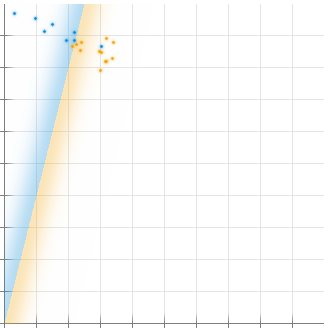
\includegraphics[width=0.99\textwidth]{example-mnist/train-plain}
            \vspace{-0.25cm}
          \caption{
            Our size-$N=25$ set of training examples, viewed in the
            darkness-height plane.  The vertical \emph{darkness} axis ranges
            $[0.0,0.25]$; the horizontal \emph{height} axis ranges $[0.0,0.5]$.
            The origin is at the lower left.  Each {\cya{cyan}} dot represents a
            $y={\cya{1}}$ example; each {\red{red}} dot, a $y={\red{9}}$ one.
            %
            The big ${\red{9}}$ above has darkness and height $(0.118, 0.375)$;\
            the big ${\cya{1}}$, $(0.092, 0.404)$.  See where they are in this
            plot?
          }
        \end{marginfigure}

        To make this precise, let's define a photo's \emph{darkness} as its
        average pixel darkness; its \emph{height} as the standard deviation of
        the row index of its dark pixels.  For convenience let's normalize
        both height and darkness to have max possible value $1.0$.  Such
        functions from inputs in $\xX$ to numbers are called
        \textbf{features}.

        \begin{lstlisting}[language=Python, basicstyle=\footnotesize\ttfamily]
          SIDE = 28
          def darkness(x):
            return np.mean(np.mean(x, axis=0), axis=0)
          def height(x):
            return np.std([row for col in range(SIDE)
                               for row in range(SIDE)
                               if 0.5 < x[row][col]  ])/(SIDE/2.0)
        \end{lstlisting}
        \par\noindent
        \attn{Exercise:} {Make a width feature.  Plot the training data
        in the height-width plane.}

        So we can threshold by darkness or by height.  But this isn't very
        satisfying, since sometimes there are especially dark ${\cya{1}}$s or
        tall ${\red{9}}$s.
        %
        We thus arrive at the idea of using \emph{both} features: ${\red{9}}$s
        are darker than ${\cya{1}}$s \emph{even relative to their
        height}.  So we might write something like
        \texttt{a*darkness(x)+b*height(x)>0} for
        %\bcirc\marginnote{%
        %  \blarr That factor of $2$ comes from our observation that darkness
        %  tends to be bigger than height.  We'll soon see that this eyeballed
        %  slope doesn't work well.  It's better to tune by machine.
        %}
        our condition.
        \par\noindent
        \attn{Exercise:} {Guess a good pair $(a,b)$ based on the training data.}
        \begin{lstlisting}[language=Python, basicstyle=\footnotesize\ttfamily]
          def hand_coded_predict(x):
            return 9 if (4.0)*darkness(x)+(-1.0)*height(x)>0 else 1
        \end{lstlisting}
        \par\noindent
        \attn{Exercise:} {Implement a crude ``hole-detector'' feature.  False
        positives are okay.}
        \par\noindent
        \attn{Exercise:} {What further features might help us to separate digits
        ${\cya{1}}$ from ${\red{9}}$?}

%~~~~~~~~~~~~~~~~~~~~~~~~~~~~~~~~~~~~~~~~~~~~~~~~~~~~~~~~~~~~~~~~~~~~~~~~~~~~~~
%~~~~~~~~~~~~~  1.4. candidate patterns  ~~~~~~~~~~~~~~~~~~~~~~~~~~~~~~~~~~~~~~

      \sampassage{candidate patterns}
        We can generalize the hand-coded hypothesis from the previous passage
        to other coefficients besides $1\cdot \text{height}(x) -
        2\cdot\text{darkness}(x)$.  We let our set $\hH$ of candidate patterns
        contain all ``linear hypotheses'' $f_{a,b}$ defined by:
        $$
          f_{a,b}(x) = {\red{9}} \text{~~if~~} a\cdot\text{darkness}(x) + b\cdot\text{height}(x) > 0 \text{~~else~~} {\cya{1}}
        $$
        Each $f_{a,b}$ makes predictions of $y$s given $x$s.  As we change $a$
        and $b$, we get different predictors, some more accurate than others.

        \begin{lstlisting}[language=Python, basicstyle=\footnotesize\ttfamily]
          def predict(x,a,b):
            return 9 if a*darkness(x) + b*height(x) > 0 else 1
        \end{lstlisting}

        \noindent
        \attn{Exercise:} {See Fig.\ \ref{fig:train-test-digits} and match up $\offourline{0}$'s $3$ lines with
        $\offourline{1}$'s $3$ boxed points.}

%~~~~~~~~~~~~~~~~~~~~~~~~~~~~~~~~~~~~~~~~~~~~~~~~~~~~~~~~~~~~~~~~~~~~~~~~~~~~~~
%~~~~~~~~~~~~~  1.5. optimization  ~~~~~~~~~~~~~~~~~~~~~~~~~~~~~~~~~~~~~~~~~~~~

      \sampassage{optimization}
        Let's write a program $\lL$ that given a list of \emph{training
        examples} produces a hypothesis in $h \in \hH$ that helps us predict
        the labels $y$ of yet-unseen photos $x$ (\emph{testing examples}).
        Insofar as training data is representative of testing data, it's
        sensible to return a $h\in \hH$ that correctly classifies maximally
        many training examples.
        %
        To do this, let's make $\lL$ loop over all integer pairs $(a,b)$ in
        $[-99,+99]$:  %to minimize the number of misclassified training examples.
        \begin{lstlisting}[language=Python, basicstyle=\footnotesize\ttfamily]
          def accuracy_on(examples,a,b):
            return sum(1.0 for x,y in examples if predict(x,a,b)==y)/len(examples)

          def best_hypothesis():
            return max((accuracy_on(training_data, a, b), (a,b))
                       for a in range(-99,100)
                       for b in range(-99,100))
        \end{lstlisting}

        \begin{figure}[h]
            \centering
            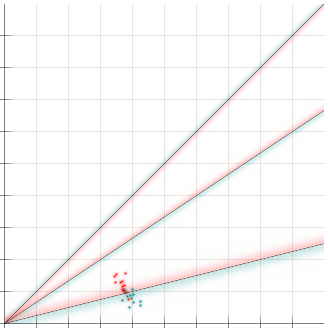
\includegraphics[width=0.23\textwidth]{example-mnist/new-train.png}%
            \hspace{0.01\textwidth}%
            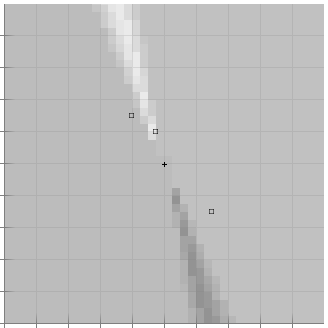
\includegraphics[width=0.23\textwidth]{example-mnist/new-train-scat.png}%
            \hspace{0.02\textwidth}%
            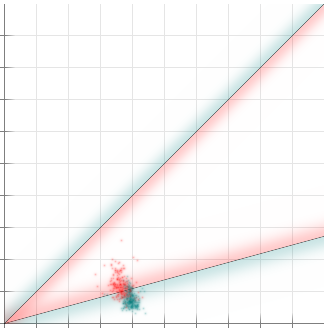
\includegraphics[width=0.23\textwidth]{example-mnist/new-test.png}%
            \hspace{0.01\textwidth}%
            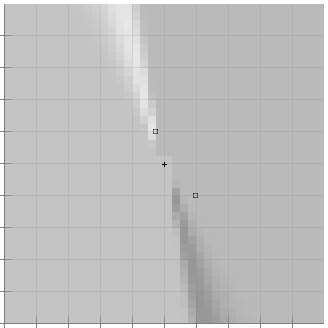
\includegraphics[width=0.23\textwidth]{example-mnist/new-test-scat.png}
            %
            \caption{
              \textbf{Training
              ($\protect\offourline{01}$) and testing
              ($\protect\offourline{23}$).}
              %
              $3$ hypotheses classify training data in the darkness-height
              plane ($\protect\offourline{0}$); glowing colors distinguish a
              hypothesis' $\cya{1}$ and $\red{9}$ sides.
              %
              Each point in the $(a,b)$ plane ($\protect\offourline{1}$)
              represents a hypothesis; darker regions misclassify a greater
              fraction of training data.
              %
              Panes $\protect\offourline{23}$ show the same for
              \emph{testing} data.
              %
              $\protect\offourline{02}$'s axes range $[0, 1.0]$.
              $\protect\offourline{13}$'s axes range $[-99,+99]$.
            }
            \label{fig:train-test-digits}
        \end{figure}


        When we feed $N=25$ training examples to $\lL$, it produces
        $(a,b)=(80,-20)$ as a minimizer of \textbf{training error}, i.e.,
        of the fraction of training examples misclassified.  It misclassifies
        only $12\%$ of training examples. Yet the same
        hypothesis misclassified a greater fraction --- $18\%$ --- of fresh,
        yet-unseen testing examples.
        %
        That latter number --- called the \textbf{testing error} --- represents
        our program's accuracy ``in the wild'';
        it's the number we most care about.  The difference between training
        and testing error is the difference between our score on a practice
        exam or homework, where we're allowed to review mistakes we made and
        do a second try, versus our score on an exam, where we don't know the
        questions beforehand and aren't allowed to change our answers once we
        get our grades back.

        \noindent
        \attn{Exercise:} {visualize $f_{a,b}$'s error on $N=1$ example as a
        function of $(a,b)$.}


